\documentclass[a4paper,12pt]{article}
\usepackage[utf8]{inputenc}
\usepackage{booktabs}
\usepackage{pgfplots}
\pgfplotsset{compat=newest}

\begin{document}
\section{V35.D.4 Minimal-LaTeX Smoke-Test}

\begin{table}[!htbp]
  \centering
  \begin{tabular}{lr}
    \toprule
    Permutation & Throughput (ops/s) \\
    \midrule
    CE-Pure-SOTA      & 1000.0 \\
    PrtArt-Innovative & 1500.0 \\
    \bottomrule
  \end{tabular}
  \caption{Sample-Tabelle Pipeline-Stage 04 Output.}
  \label{tab:v35d4_minimal}
\end{table}

\begin{figure}[!htbp]
  \centering
  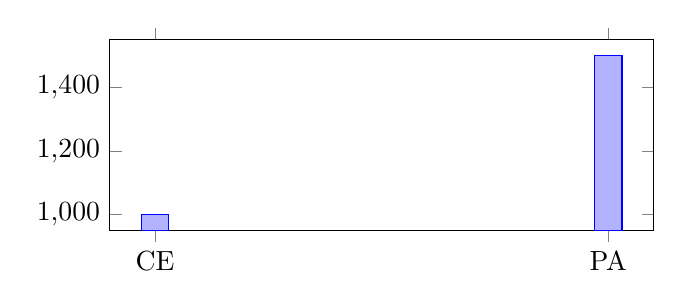
\begin{tikzpicture}
    \begin{axis}[width=0.7\textwidth,height=4cm,ybar,symbolic x coords={CE,PA},xtick=data]
      \addplot+[] coordinates {(CE,1000) (PA,1500)};
    \end{axis}
  \end{tikzpicture}
  \caption{Sample-TikZ Pipeline-Stage 05 Output.}
  \label{fig:v35d4_minimal}
\end{figure}

\end{document}
